\documentclass[15pt, a4paper]{article}
\usepackage[T1]{fontenc}
\usepackage[polish]{babel}
\usepackage[utf8]{inputenc}
\usepackage{tikz}
\usepackage{adjustbox}
\usepackage{longtable}
\usepackage{graphicx}
\usepackage{amsfonts}
\title{Obliczenia naukowe}
\author{Felix Zieliński 272336}
\date{Lista 2}
\begin{document}
\maketitle
TODO OPIS, czy zadanie 2? CO SIE STALO Z GNUPLOTEM zadanie 3, ta bogusowa tabela w 4, zadanie 5 opis i wnioski, zadanie 6, opisy funkcji, wnioski koncowe, wszystkie bogusowe tabele i obrazki

\vspace{0.5cm}

\noindent\hrulefill

% zadanie 1

\vspace{0.5cm}

\noindent\textbf{Zadanie 1.} Niewielkie zmiany danych oraz ich wpływ na wyniki obliczeń.\\

\noindent W ramach przypomnienia zadania: na poprzedniej liście  należało obliczyć iloczyny skalarne dwóch wektorów na cztery rózne sposoby.\\\\
Zaimplementowałem każdy z podanych w poleceniu sposobów, tak więc funkcja \verb|a| liczy "w przód", od pierwszych indeksów, funkcja \verb|b| "w tył", analogicznie, a \verb|c| oraz \verb|d| liczą, odpowiednio, od największego do najmniejszego oraz od najmniejszego do największego względem ich wartości absolutnej.\\\\
Różnica w tym zadaniu, a zadaniu 5. z poprzedniej listy polegała na dokonaniu drobnej zmiany w niektórych wartościach wektora. Poniżej prezentuję wyniki otrzymane po, jak i przed tej zmianie:


\begin{table}[ht]
    \begin{adjustbox}{max width=\textwidth}
    \begin{tabular}{|c|c|c|c|c|}
        \hline 
        Sposób & Float32 stare & Float32 nowe & Float64 stare & Float64 nowe \\ \hline
        a & -0.4999443 & -0.4999443 & 1.0251881368296672e-10 & -0.004296342739891585 \\ \hline
        b & -0.4543457 & -0.4543457 & -1.5643308870494366e-10 & -0.004296342998713953 \\ \hline
        c & -0.5 & -0.5 & 0.0 & -0.004296342842280865 \\ \hline
        d & -0.5 & -0.5 & 0.0 & -0.004296342842280865 \\ \hline
    \end{tabular}
    \end{adjustbox}
    \caption{Porównanie nowych i starych danych}
    \label{tab:products}
\end{table}

\vspace{0.5cm}

\noindent gdzie wartość prawidłowa wynosi: \[\verb|-1.00657107000000e-11|\]

Jak widać, wyniki dla typu \verb|Float32| nie zmieniły się. Jest to spowodowane niewystarczającą do zauważenia różnicy precyzją zapisu liczby zmiennopozycyjnej w tym typie.\\\\
Natomiast w typie \verb|Float64| różnica jest znaczna mimo tak niewielkiej zmiany danych. Mimo że wyniki nadal odbiegają od prawidłowego, są one mu znacznie bliższe. \\\\
Można więc stwierdzić, że zadanie to było \textbf{źle uwarunkowane} - o wysokim wskaźniku uwarunkowania. Wskaźnik ten określa, w jakim stopniu błąd reprezentacji numerycznej danych wejściowych dla danego problemu będzie wpływać na błąd wyniku. Małe zmany danych w tym zadaniu spowodowały znaczną zmianę wyników. 

\vspace{0.5cm}

\noindent\hrulefill

% zadanie 2

\vspace{0.5cm}

\noindent\textbf{Zadanie 2.} W tym zadaniu należało narysować wykres funkcji \[f(x) = e^{x}\ln(1 + e^{-x})\] 
w dwóch różnych programach do wizualizacji danych. Zdecydowałem się na użycie WolframaAlpha, Desmosa oraz Gnuplota

\begin{figure}[h]
    \centering
    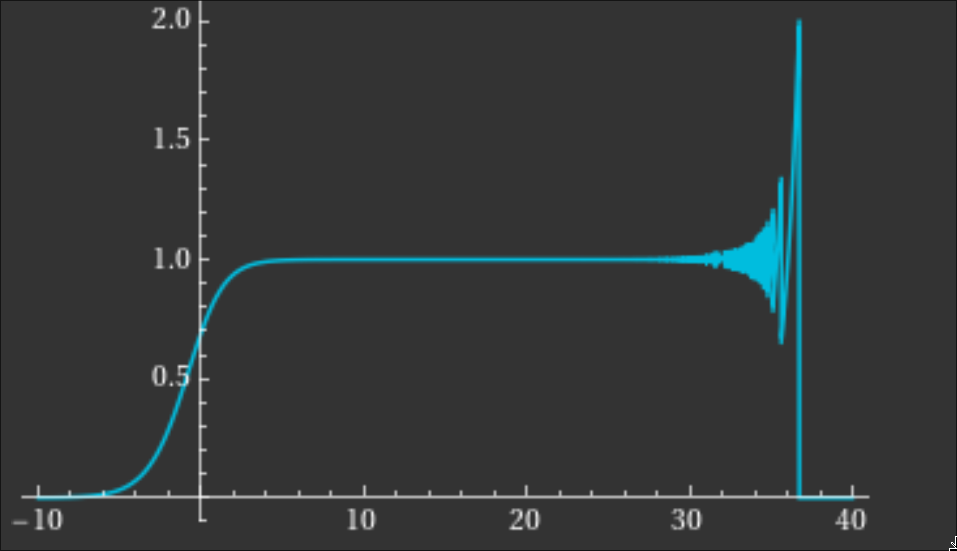
\includegraphics[width=0.5\textwidth]{img/wolfram1.png}  
    \caption{WolframAlpha: \texttt{plot $e^{x} * \ln(1 + e^{-x})$ from $x = -10$ to $x = 40$}}
\end{figure}

\begin{figure}[h]
    \centering
    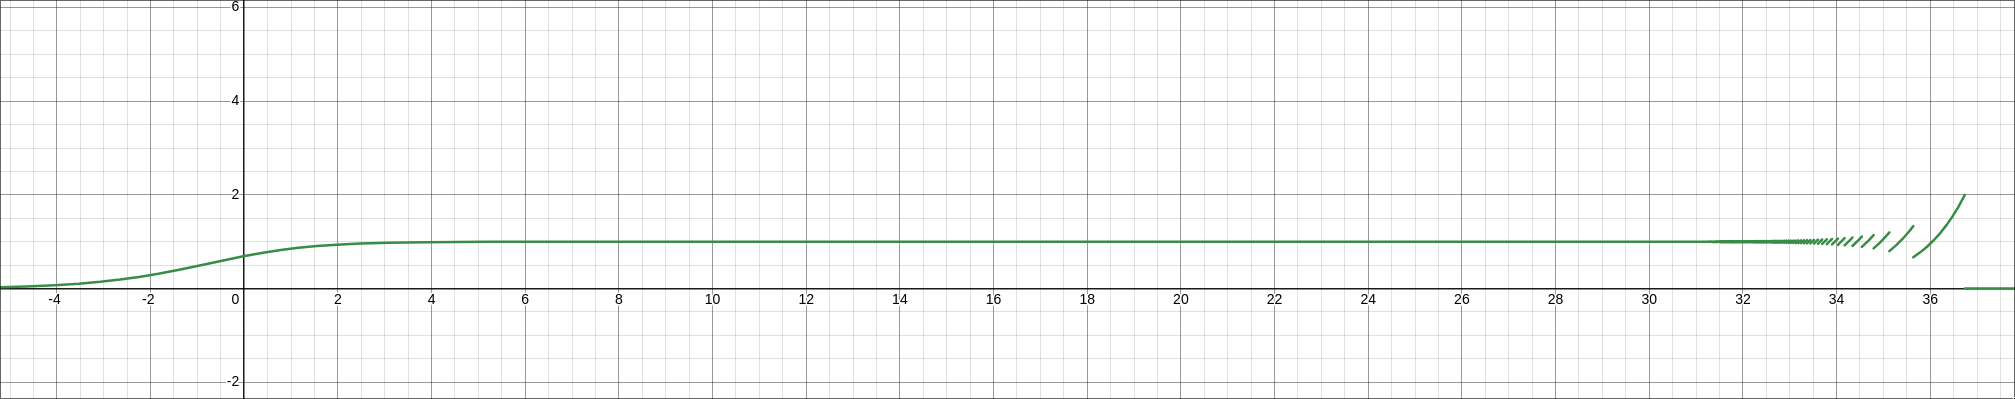
\includegraphics[width=0.5\textwidth]{img/desmos1.png}
    \caption{Desmos}
\end{figure}

\begin{figure}[h]
    \centering
    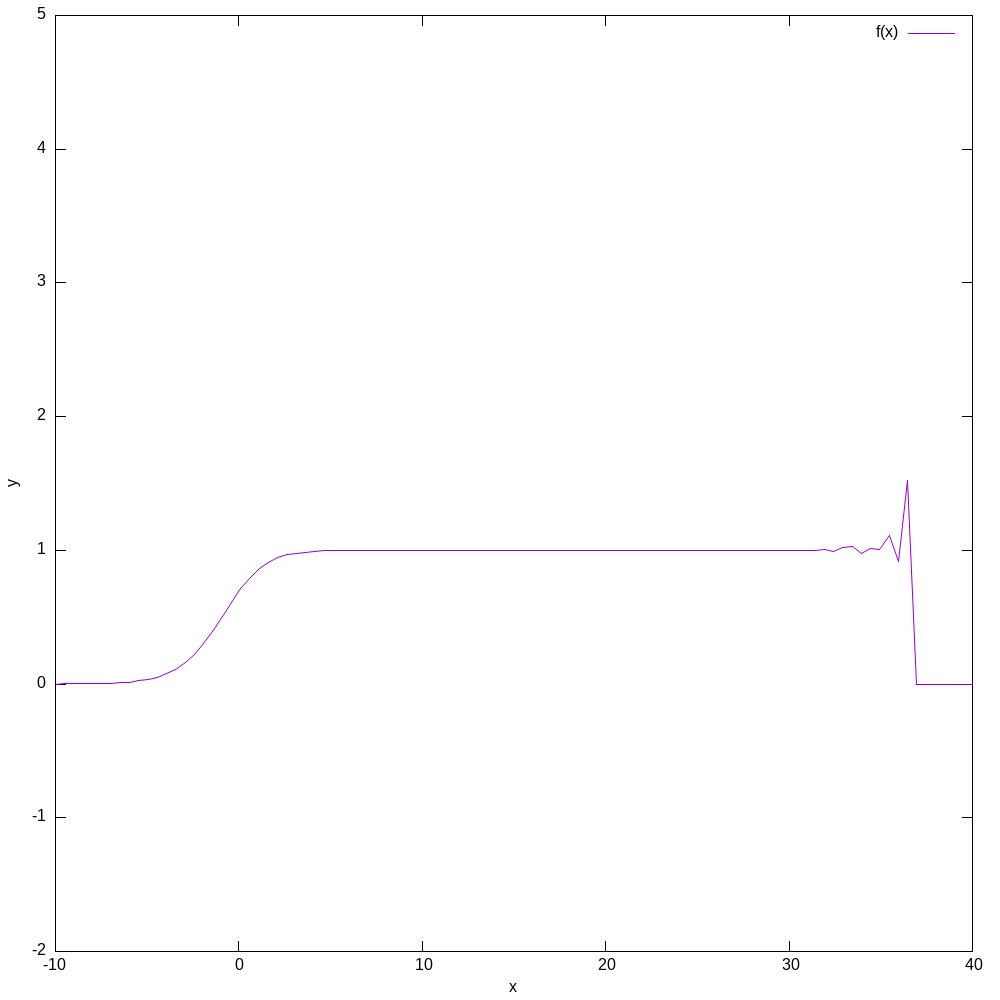
\includegraphics[width=0.5\textwidth]{img/gnuplot1.png}
    \caption{Gnuplot}
\end{figure}

\vspace{0.5cm}

\noindent Granica tej funkcji dla x zmierzającego do nieskończoności wynosi 

\[
\lim_{x \to \infty} f(x) = \lim_{x \to \infty} e^x \ln(1 + e^{-x}) = 1
\]

\noindent Jak można zauważyć, dla wartości \verb|x >= 32| wykresy zaczynają wskazywać błędne wartości, każdy na trochę inny sposób. Oscylują one wokół 1, coraz bardziej odbiegając od jej wartości, a następnie spadają do 0. \\\\

\noindent Dzieje się tak, gdyż dla \verb|x > 30| wartości $e^{x}$ są już tak duże, że mnożenie jej z niewielką wartością $ln(1 + e^{-x})$ skutkuje znacznymi błędami przybliżenia, które dla ok \verb|x = 38| powodują zwracanie wartości 0. Jest to spowodowane przybliżeniem $1 + e^{-x} \approx 1$, i tym samym całej wartości logarytmu do 0. Tak więc algorytm obliczający wartości \verb|f(x)| nie jest stabilny numerycznie.

\vspace{0.5cm}

\noindent\hrulefill

% zadanie 3

\vspace{0.5cm}

\noindent\textbf{Zadanie 3.} W zadaniu tym należało rozwiązać liniowy układ równań \verb|A * x = b| dla danej macierzy współczynników \( A \in \mathbb{R}^{n \times n} \) i wektora prawych stron \( b \in \mathbb{R}^n \). Macierze były generowane poprzez dostarczone przez prowadzącego funkcje: generującą macierz Hilberta \verb|n|-tego stopnia oraz generującą losową macierz \verb|n|-tego stopnia z zadanym wskaźnikiem uwarunkowania.\\\\
W tabelach przedstawiłem błędy względne dla zadanych algorytmów: eliminacji Gaussa oraz inwersji. Uwarunkowanie oraz rząd macierzy są obliczanie poprzez wbudowane w paczkę LinearAlgebra funkcje \verb|cond()| oraz \verb|rank()|.

\vspace{0.5cm}

\begin{table}[ht]
    \begin{adjustbox}{max width=\textwidth}
    \begin{tabular}{|c|c|c|c|c|}
        \hline 
        n & uwarunkowanie & rząd & błąd metody Gaussa & błąd metody inwersji \\ \hline
        1  & 1.0                & 1  & 0.0                           & 0.0                           \\ \hline
        2  & 19.281470067903967 & 2  & 5.661048867003676e-16         & 1.1240151438116956e-15       \\ \hline
        3  & 524.0567775860627  & 3  & 8.351061872731819e-15         & 9.825526038180824e-15        \\ \hline
        4  & 15513.738738929662 & 4  & 4.2267316576255873e-13        & 3.9600008750140806e-13       \\ \hline
        5  & 476607.2502419338  & 5  & 1.256825919192874e-12         & 8.128168770215688e-12        \\ \hline
        6  & 1.495105864177819e7 & 6  & 1.5435074657413347e-10       & 1.0423794065751672e-10       \\ \hline
        7  & 4.753673568766496e8 & 7  & 6.520804933066021e-9         & 4.3299229851434615e-9        \\ \hline
        8  & 1.5257575563722723e10 & 8 & 3.6010489197068436e-7       & 4.0236799996435915e-7        \\ \hline
        9  & 4.9315332284138226e11 & 9 & 1.3216991540025553e-5       & 1.4626798972086921e-5        \\ \hline
        10 & 1.6024980732174455e13 & 10 & 0.0004194170177181955      & 0.00040714905218460087       \\ \hline
        11 & 5.224780779168285e14  & 10 & 0.01004906783345069        & 0.010645959401385671         \\ \hline
        12 & 1.6425917529444498e16 & 11 & 0.5502106922296848         & 0.6697890564301745           \\ \hline
        13 & 4.4936679531246986e18 & 11 & 70.1556197115221           & 82.66675811171989            \\ \hline
        14 & 3.2198422552156205e17 & 11 & 9.649642437452474          & 10.094732062453225           \\ \hline
        15 & 3.3660126672602944e17 & 12 & 692.4295360390742          & 715.740988667373             \\ \hline
        16 & 2.249940193352714e18  & 12 & 10.414656083840297         & 8.442143351389534            \\ \hline
        17 & 6.26204622473199e17   & 12 & 18.67581817300634          & 17.157982115668773           \\ \hline
        18 & 3.266632306940269e18  & 12 & 5.40548300394664           & 3.742412802776696            \\ \hline
        19 & 3.462302955915255e18  & 13 & 15.073941146224387         & 16.84769281513296            \\ \hline
        20 & 6.806966421072721e18  & 13 & 28.79267493699834 & 30.751202239608727           \\ \hline
           \end{tabular}
    \end{adjustbox}
    \label{tab:hilbert}
    \caption{Macierze Hilberta}
\end{table}

\noindent Im wyższe uwarunkowanie, tym wyższy błąd względny dla obu metod.

\vspace{0.5cm}


\begin{table}[ht]
    \begin{adjustbox}{max width=\textwidth}
    \begin{tabular}{|c|c|c|c|c|c|}
        \hline 
        n & c & uwarunkowanie & rząd & błąd metody Gaussa & błąd metody inwersji \\ \hline
        5 & $10^0$ & 1.0000000000000007 & 5 & 2.0471501066083611e-16 & 1.7901808365247238e-16 \\ \hline
        5 & $10^1$ & 10.00000000000001 & 5 & 2.579925170969555e-16 & 1.4895204919483638e-16 \\ \hline
        5 & $10^3$ & 999.9999999999956 & 5 & 4.154180998732242e-14 & 3.6649738390350505e-14 \\ \hline
        5 & $10^7$ & 9.999999992624711e6 & 5 & 1.2808136131610903e-10 & 1.2922561774440224e-10 \\ \hline
        5 & $10^{12}$ & 1.0000402198324714e12 & 5 & 2.4114718692896424e-5 & 2.1083207553058387e-5 \\ \hline
        5 & $10^{16}$ & 6.457380316295465e15 & 4 & 0.279866038431425 & 0.23511506127614903 \\ \hline
        10 & $10^0$ & 1.0000000000000009 & 10 & 3.1006841635969763e-16 & 2.6506211417561425e-16 \\ \hline
        10 & $10^1$ & 9.999999999999991 & 10 & 2.432376777795247e-16 & 3.255813018879823e-16 \\ \hline
        10 & $10^3$ & 999.9999999999854 & 10 & 5.123291327463699e-15 & 4.80612456985904e-15 \\ \hline
        10 & $10^7$ & 9.99999999300524e6 & 10 & 2.613887510795298e-10 & 2.9367939862640613e-10 \\ \hline
        10 & $10^{12}$ & 9.999916908430352e11 & 10 & 2.5298084239916387e-5 & 2.7222350440303e-5 \\ \hline
        10 & $10^{16}$ & 5.260556228219448e16 & 9 & 0.2349713562983511 & 0.17164964730117435 \\ \hline
        20 & $10^0$ & 1.0000000000000009 & 20 & 5.450279209566124e-16 & 4.557326905135503e-16 \\ \hline
        20 & $10^1$ & 9.99999999999999 & 20 & 5.318651993048588e-16 & 3.430930459816227e-16 \\ \hline
        20 & $10^3$ & 1000.0000000000724 & 20 & 4.374127960791212e-14 & 3.7395403352225206e-14 \\ \hline
        20 & $10^7$ & 1.0000000008586796e7 & 20 & 4.8148086460727405e-12 & 7.333934288678081e-11 \\ \hline
        20 & $10^{12}$ & 1.000058179546536e12 & 20 & 5.063442743791289e-5 & 5.134232142086649e-5 \\ \hline
        20 & $10^{16}$ & 9.35903000507404e15 & 19 & 0.13171344480426542 & 0.16281145033250885 \\ \hline
    \end{tabular}
    \end{adjustbox}
    \caption{Macierze losowe}
    \label{tab:inversion}
\end{table}

\vspace{0.5cm}

\noindent Tak jak przy macierzach Hilberta, w wynikach dla macierzy losowych można zaobserwować rosnący błąd względny. Ponadto widać, że funkcja cond() nie oblicza dokładnie uwarunkowania, tylko je przybliża. Ponadto wartości tych przybliżeń są różne dla różnych procesorów. \\\\
\noindent Powyższe tabele pozwalają na wyciągnięcie wniosku, że zadanie to było źle uwarunkowane, zwłaszcza dla macierzy Hilberta - wraz ze wzrostem stopnia macierzy ostro rośnie też wskaźnik uwarunkowania i, jednocześnie, błąd względny. Dla macierzy losowych dzieje się podobnie, jednakże ten wzrost jest wolniejszy (błędy są mniejsze).

\vspace{0.5cm}

\noindent\hrulefill

% zadanie 4

\vspace{0.5cm}

\noindent\textbf{Zadanie 4.} W zadaniu tym należało obliczyć miejsca zerowe zadanego wielomianu \verb|P(x)| i przedstawić wyniki dla \( z_k \), \( 1 \leq k \leq 20 \), obliczając \( |P(z_k)| \), \( |p(z_k)| \) i \( |z_k - k| \). Następnie należało powtórzyć eksperyment Wilkinsona, czyli lekko zmodyfikować wielomian i przeprowadzić ponownie obliczenia.

\vspace{0.5cm}

\begin{table}[h]
    \begin{adjustbox}{max width=\textwidth}
    \begin{tabular}{|c|c|c|c|c|}
        \hline
        \(k\) & \(z_k\) & \(|Pz_k|\) & \(|pz_k|\) & \(|z_k - k|\) \\ \hline
           \end{tabular}
    \end{adjustbox}
    \label{wielomian}
    \caption{Wielomian P(x)}
\end{table}

\vspace{0.5cm}

\noindent Jak można zauważyć, obliczone miejsca zerowe przy pomocy \verb|roots()| są zbliżone, ale nie równe wartościom prawidłowym.

\vspace{0.5cm}

\noindent\hrulefill

% zadanie 5

\vspace{0.5cm}

\noindent\textbf{Zadanie 5.}  

\begin{longtable}{|c|c|c|c|}
        \hline
        n & 1. eksperyment & 2. eksperyment (z obcięciem) & 3. eksperyment (Float64) \\ \hline
        0 & 0.01 & 0.01 & 0.01 \\ \hline
        1 & 0.0397 & 0.0397 & 0.0397 \\ \hline
        2 & 0.15407173 & 0.15407173 & 0.15407173000000002 \\ \hline
        3 & 0.5450726 & 0.5450726 & 0.5450726260444213 \\ \hline
        4 & 1.2889781 & 1.2889781 & 1.2889780011888006 \\ \hline
        5 & 0.1715188 & 0.1715188 & 0.17151914210917552 \\ \hline
        6 & 0.5978191 & 0.5978191 & 0.5978201201070994 \\ \hline
        7 & 1.3191134 & 1.3191134 & 1.3191137924137974 \\ \hline
        8 & 0.056273222 & 0.056273222 & 0.056271577646256565 \\ \hline
        9 & 0.21559286 & 0.21559286 & 0.21558683923263022 \\ \hline
        10 & 0.7229306 & 0.7229306 & 0.722914301179573 \\ \hline
        11 & 1.3238364 & 1.3241479 & 1.3238419441684408 \\ \hline
        12 & 0.037716985 & 0.036488414 & 0.03769529725473175 \\ \hline
        13 & 0.14660022 & 0.14195944 & 0.14651838271355924 \\ \hline
        14 & 0.521926 & 0.50738037 & 0.521670621435246 \\ \hline
        15 & 1.2704837 & 1.2572169 & 1.2702617739350768 \\ \hline
        16 & 0.2395482 & 0.28708452 & 0.24035217277824272 \\ \hline
        17 & 0.7860428 & 0.9010855 & 0.7881011902353041 \\ \hline
        18 & 1.2905813 & 1.1684768 & 1.2890943027903075 \\ \hline
        19 & 0.16552472 & 0.577893 & 0.17108484670194324 \\ \hline
        20 & 0.5799036 & 1.3096911 & 0.5965293124946907 \\ \hline
        21 & 1.3107498 & 0.09289217 & 1.3185755879825978 \\ \hline
        22 & 0.088804245 & 0.34568182 & 0.058377608259430724 \\ \hline
        23 & 0.3315584 & 1.0242395 & 0.22328659759944824 \\ \hline
        24 & 0.9964407 & 0.94975823 & 0.7435756763951792 \\ \hline
        25 & 1.0070806 & 1.0929108 & 1.315588346001072 \\ \hline
        26 & 0.9856885 & 0.7882812 & 0.07003529560277899 \\ \hline
        27 & 1.0280086 & 1.2889631 & 0.26542635452061003 \\ \hline
        28 & 0.9416294 & 0.17157483 & 0.8503519690601384 \\ \hline
        29 & 1.1065198 & 0.59798557 & 1.2321124623871897 \\ \hline
        30 & 0.7529209 & 1.3191822 & 0.37414648963928676 \\ \hline
        31 & 1.3110139 & 0.05600393 & 1.0766291714289444 \\ \hline
        32 & 0.0877831 & 0.21460639 & 0.8291255674004515 \\ \hline
        33 & 0.3280148 & 0.7202578 & 1.2541546500504441 \\ \hline
        34 & 0.9892781 & 1.3247173 & 0.29790694147232066 \\ \hline
        35 & 1.021099 & 0.034241438 & 0.9253821285571046 \\ \hline
        36 & 0.95646656 & 0.13344833 & 1.1325322626697856 \\ \hline
        37 & 1.0813814 & 0.48036796 & 0.6822410727153098 \\ \hline
        38 & 0.81736827 & 1.2292118 & 1.3326056469620293 \\ \hline
        39 & 1.2652004 & 0.3839622 & 0.0029091569028512065 \\ \hline
        40 & 0.25860548 & 1.093568 & 0.011611238029748606 \\ \hline
    \caption{Model logistyczny - wyniki}
\end{longtable}

\vspace{0.5cm}

\noindent\hrulefill

% zadanie 6
 
\vspace{0.5cm}


\noindent\textbf{Zadanie 6.} W zadaniu tym, podobnie jak w poprzednim, należało rozważyć równanie rekurencyjne  
\[
    x_{n+1} := x_n^2 + c \quad \mathrm{dla} \quad n = 0, 1, \ldots
\]
Należało, w arytmetyce \verb|Float64|, iterować 40-sto krotnie powyższe równanie, z różnymi wartościami początkowymi \verb|x| oraz \verb|c|. Poniżej znajdują się reprezentacje graficzne, wykonane przy pomocy paczki Plots języka Julia, dla poszczególnych wartości.

\vspace{0.5cm}

\begin{figure}[h]
    \centering
    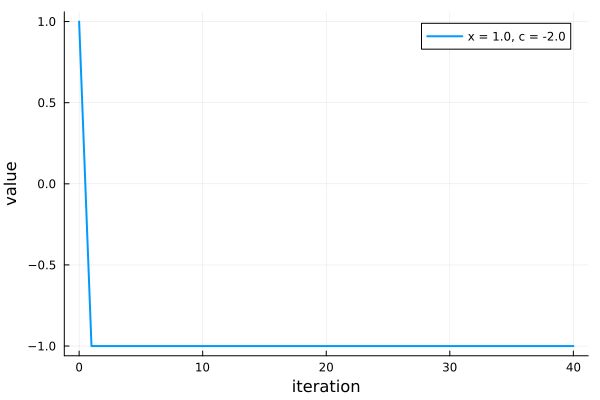
\includegraphics[width=0.7\textwidth]{img/6_1_plot.png}
\end{figure}

\begin{figure}[h]
    \centering
    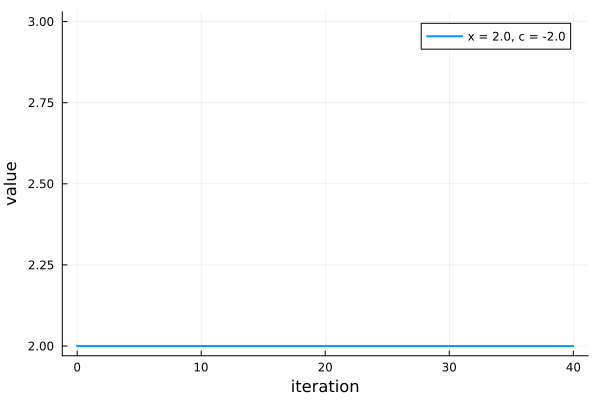
\includegraphics[width=0.7\textwidth]{img/6_2_plot.png}
\end{figure}

\vspace{0.5cm}

\noindent Powyższe wykresy są są stałe.

\vspace{0.5cm}

\begin{figure}[h]
    \centering
    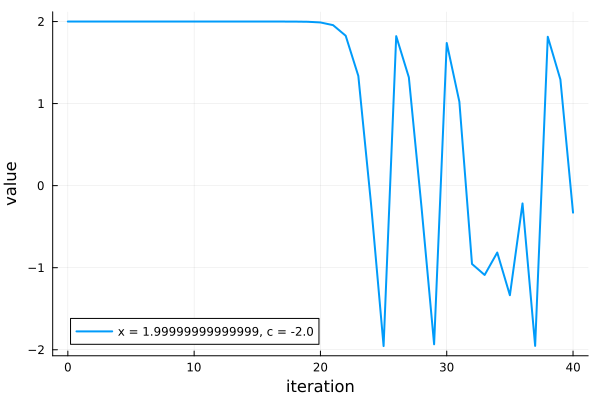
\includegraphics[width=0.7\textwidth]{img/6_3_plot.png}
\end{figure}

\vspace{0.5cm}

\noindent Dla wykresu z \verb|x = 1.99999999999999|, po pewnym czasie otrzymujemy bardzo niepoprawne wyniki, mniejsze od 2, chociaż, według intuicji, powinny one być bliskie 2.

\vspace{0.5cm}

\begin{figure}[h]
    \centering
    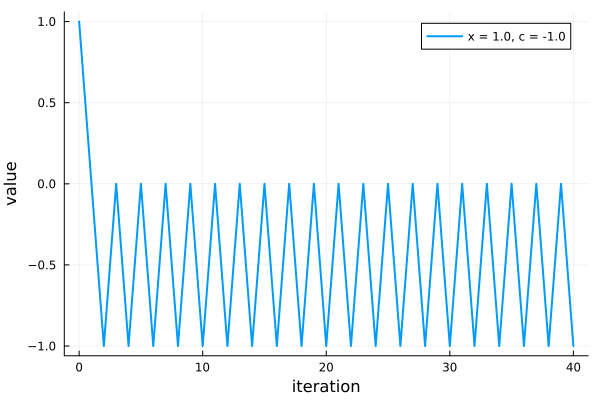
\includegraphics[width=0.7\textwidth]{img/6_4_plot.png}
\end{figure}

\begin{figure}[h]
    \centering
    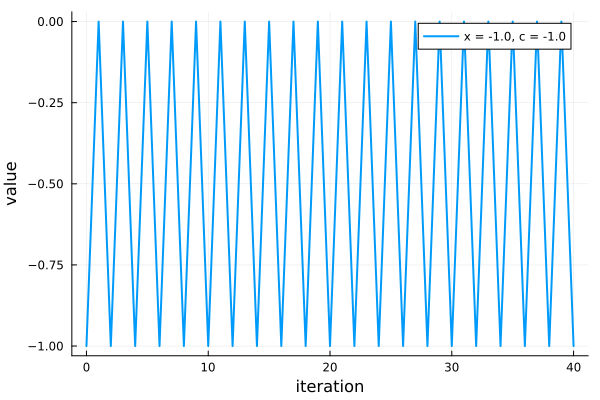
\includegraphics[width=0.7\textwidth]{img/6_5_plot.png}
\end{figure}

\vspace{0.5cm}

\noindent Dla powyższych wykresów, wyniki są stabilne, oscylują wokół przewidywanych wartości.

\vspace{0.5cm}

\begin{figure}[h]
    \centering
    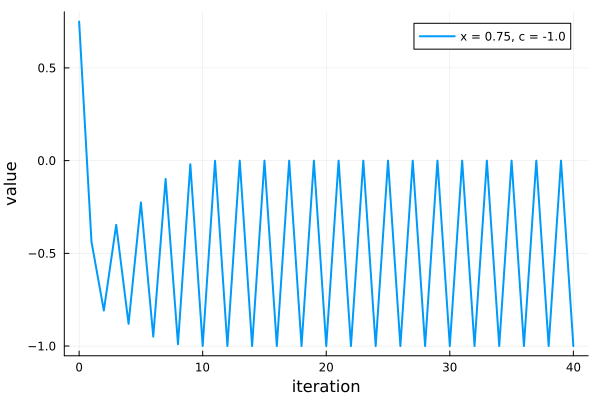
\includegraphics[width=0.7\textwidth]{img/6_6_plot.png}
\end{figure}

\begin{figure}[h]
    \centering
    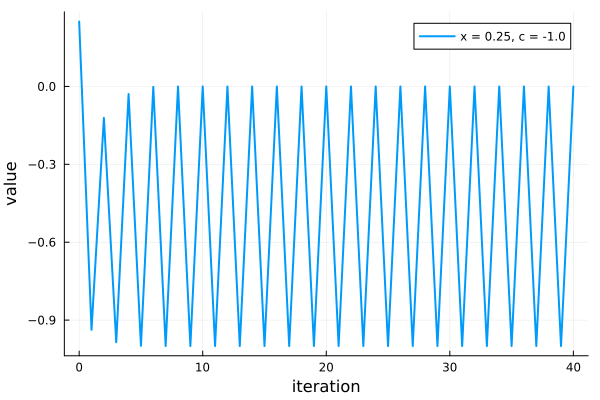
\includegraphics[width=0.7\textwidth]{img/6_7_plot.png}
\end{figure}

\vspace{0.5cm}

\noindent Wykresy dla \verb|x = 0.75| oraz \verb|x = 0.25| po czasie stabilizują się i przyjmują, na zmianę, wartości -1 oraz 0.

\vspace{0.5cm}

\noindent Fakt, że dokładność arytmetyki liczb zmiennopozycyjnych jest skończona, wpływa na wyniki (wykresy dla \verb|x = 0.75| oraz \verb|x = 0.25|, które zaczynają zbiegać do liczb całkowitych).  Ponadto kumulowanie się błędu (jak podczas obliczeń z \verb|x = 1.99999999999999|) powoduje znaczące odbieganie wyników od ich wartości prawidłowej. Gdy \verb|x| jest liczbą całkowitą, wyniki zachowują się poprawnie.\\\\
Niewielkie zmiany w danych prowadzą w tym zadaniu do róznych wyników - możemy wnioskować, że jest to zadanie źle uwarunkowane.

\end{document}
